\subsection{TMC4671-EVAL Board}\label{subsec:TMC4671_EVAL_Boad}

Wie bereits angesprochen steuert der TMC4671 die Kommuntierungsvorgänge für den BLDC. Doch er ist noch zu viel mehr in der Lage. Der TMC4671 ist ein voll integrierter Servo-Controller, der eine feldorientierte Steuerung für BLDC/PMSM, 2-Phasen-Schrittmotoren und DC-Motoren unterstützt. Ob integrierte ADCs, Lagesensor-Schnittstellen oder Positionsinterpolatoren, alle diese in der Hardware implementierten Steuerungsfunktionen bieten einen voll funktionsfähigen Servoregler für ein breites Spektrum an Servoanwendungen. \cite{trinamic_datasheet_2018}

\subsubsection{Aufbau}\label{subsubsec:TMC4671_Aufbau}

Das komplette EVAL-Board, wie es in Abbildung \ref{fig:TMC4671_EVAL_Board} gezeigt wird, besteht aus einer Landungsbrücke (links), einem TMC4671 (mitte) und einer H-Brücke (rechts). Verbunden werden die drei Teile mittels zwei Eselsbrücken.

\begin{figure}[h!]
	\centering
	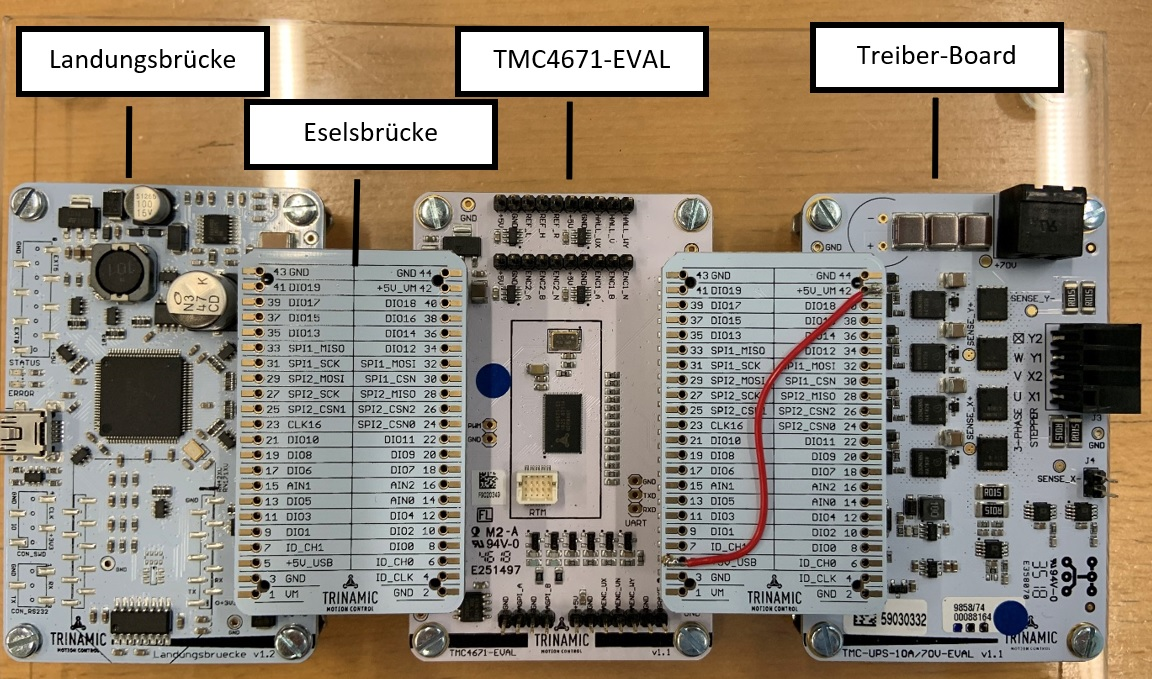
\includegraphics[width=0.6\textwidth]{graphics/TMC4671_EVAL.jpg}
	\caption{TMC4671-EVAL Board. 
	\cite{unbekannt_foc-motorenansteuerung_2019}
	}
	\label{fig:TMC4671_EVAL_Board}
\end{figure}

Die Landungsbrücke verfügt über einen USB-Anschluss, um vom Computer aus auf die Landungsbrücke zugreifen zu können. Sie bildet somit die Schnittstelle zwischen der TMCL-IDE und dem Motorentreiber, worüber die Konfiguration des Treibers stattfindet.
Der Motorentreiber stellt anhand der Konfigurationen und des Feedbacks (Spulenströme und Encodersignale) die Steuersignale für den Gate-Treiber bereit.
Der Gate-Treiber steuert die Spulenströme und magnetisiert so die Spulen des BLDC-Motors anhand der Steuersignale des Treibers. Dies wiederum verursacht eine Bewegung des Rotors.

\subsubsection{FOC}

FOC\footnote{FOC = \textbf{F}ield \textbf{O}riented \textbf{C}ontrol} ist ein Stromregelverfahren für Elektromotoren. Es reguliert die Kraft und Lage des magnetischen Feldes unter Berücksichtigung der Rotorposition, sodass der Motor das geforderte Drehmoment als Soll-Drehmoment abgibt.
FOC maximiert die Wirkleistung und minimiert die Leerlaufleistung. Dies wiederum ergibt eine Verminderung der Verlustleistung durch
intelligente Regelung. \cite{trinamic_datasheet_2018}

Auf den Rotor eines BLDC-Motors wirken zwei Kraftkomponenten. Gemäss Abbildung \ref{fig:TMC4671_EVAL_Board_FOC1} zieht eine Komponente radial in eine Richtung $I_D$ und eine andere Komponente tangential in eine Richtung $I_Q$. Die zweite Komponente $I_Q$ ist diejenige, welche ein Drehmoment auf den Rotor bringt. Der ideale Controller führt eine Regelung durch, welche einen rein drehmomenterzeugenden Strom $I_Q$ erzeugt. \cite{trinamic_datasheet_2018}

\begin{figure}[h!]
	\centering
	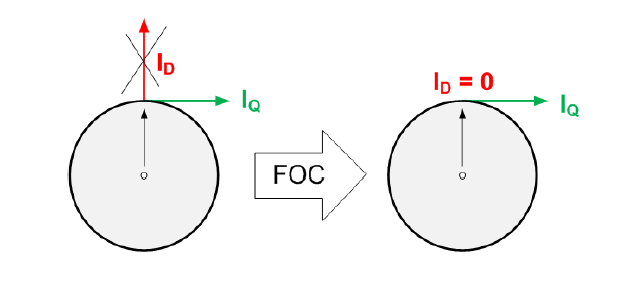
\includegraphics[width=0.6\textwidth]{graphics/FOC1.png}
	\caption{TMC4671-EVAL Board. \cite{trinamic_datasheet_2018}}
	\label{fig:TMC4671_EVAL_Board_FOC1}
\end{figure}

Der Controller verwendet für das Stromregelverfahren die drei Phasenströme des Stators, welche zusammen als Vektor betrachtet werden ($I_{U}$,$I_{V}$,$I_{W}$).
Unter Berücksichtigung der momentanen Ausrichtung des Rotors wird ein Spannungsvektor ($U_{U}$,$U_{V}$,$U_{W}$)  berechnet, sodass nur ein drehmomentbildender Strom $I_Q$ erzeugt wird (Transformation). \cite{trinamic_datasheet_2018}

Dazu sind einige statische Parameter nötig, wie z.B die Polpaarzahl des Motors, Anzahl der Impulse pro Umdrehung des verwendeten Drehgebers. Aber auch einige dynamische Parameter wie z.B die Phasenströme oder die Orientierung des Rotors. \cite{trinamic_datasheet_2018}

Von Bedeutung sind die Einstellungen der P und I Parameter zur Regelung der Phasenströme. Diese sind abhängig von den elektrischen Parametern des Motors wie z.B der Widerstand, die Induktivität, die Gegen-EMF-Konstante oder die Versorgungsspannung. \cite{trinamic_datasheet_2018}

Abbildung \ref{fig:Blockdiagramm_TMC4671} zeigt, an welcher Stelle im TMC4671 FOC (FOC23) aktiv ist. Wie zu erkennen ist, steht es mit fast allen Teilsystemen in Kontakt.
\\

\begin{figure}[h!]
	\centering
	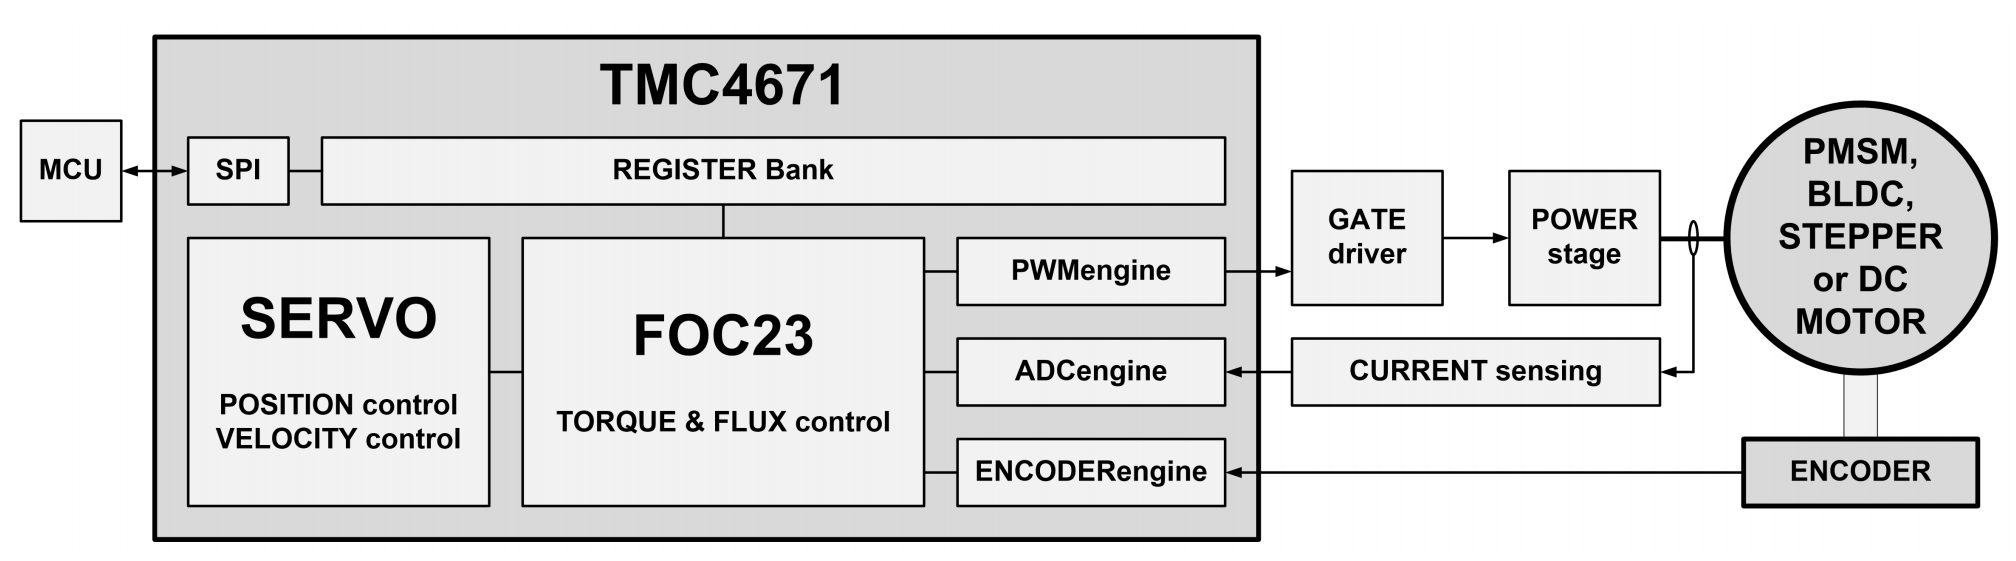
\includegraphics[width=0.7\textwidth]{graphics/Blockdiagramm_TMC4671.png}
	\caption{Standard-Anwendungs-Schaltung. \cite{trinamic_datasheet_2018}}
	\label{fig:Blockdiagramm_TMC4671}
\end{figure}
\newpage

\subsubsection{Park \& Clarke}

Für das Stromregelverfahren werden die Funktionen Clarke, Park, iClarke und iPark verwendet. Im Folgenden wird gezeigt, wie sie im Zusammenhang mit dem drehmomentgebenden Strom, den Phasenströmen, den Phasenspannungen und den PI-Parameter stehen. In Abbildung \ref{fig:TMC4671_EVAL_Board_Park_and_Clarke} sind die Zusammenhänge grafisch dargestellt.

%\begin{tabular}{lll}
%Statorströme \textbf{($I_{U}$,$I_{V}$,$I_{W}$)}& Clarke &  Stromvektor der drei Statorströme ($I_\alpha$,$I_\beta$)\\
%Stromvektor Stator ($I_\alpha$,$I_\beta$) & Park & Momentaner Stromvektor auf Rotor ($I_Q$,$I_D$)  \\
%Stromvektor Rotor ($I_Q$,$I_D$) & PID &  Berechnete Spannungen für Rotor ($U_Q$,$U_D$)\\
%Rotorspannungen ($U_Q$,$U_D$) & iPark &  Spannungsvektor der drei Statorspannungen ($U_\alpha$,$U_\beta$)\\
%Spannungsvektor ($U_\alpha$,$U_\beta$) & iClarke &  Statorspannungen \textbf{($U_{U}$,$U_{V}$,$U_{W}$)} \\
%\end{tabular}

\begin{figure}[h!]
	\centering
	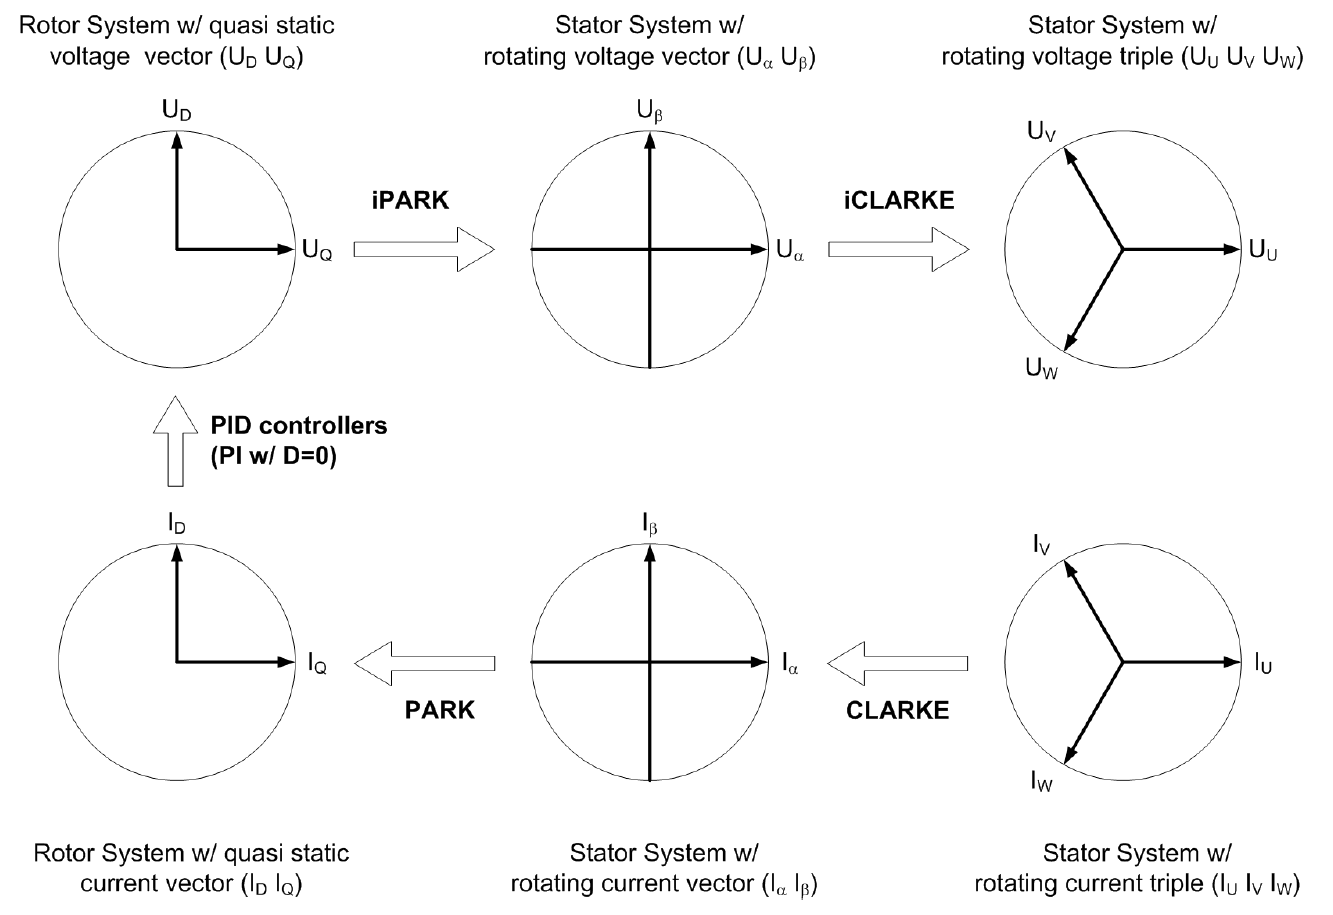
\includegraphics[width=\textwidth]{graphics/PI_Regler_Park_and_Clarke.png}
	\caption{TMC4671-EVAL Board. \cite{trinamic_datasheet_2018}}
	\label{fig:TMC4671_EVAL_Board_Park_and_Clarke}
\end{figure}

Die Clarke-Transformation (CLARKE) bildet drei Motorphasenströme ($I_{U}$,$I_{V}$,$I_{W}$) auf ein zweidimensionales
Koordinatensystem mit zwei Strömen ($I_\alpha$,$I_\beta$) ab. Basierend auf dem tatsächlichen Rotorwinkel, der durch einen Encoder oder über eine sensorlose Elektronik ermittelt wird, bildet die Park-Transformation (PARK) diese beiden Ströme auf ein näherungsweise statisches
Koordinatensystem mit zwei Strömen ($I_Q$,$I_D$) ab. Der aktuelle Strom $I_D$ steht für den Flux und der aktuelle Strom $I_Q$ für das Drehmoment. Der Flux zieht nur am Rotor, beeinflusst aber das Drehmoment nicht. Das Drehmoment wird durch den Strom $I_Q$ beeinflusst.
Zwei PI Regler ($PID_Q$, $PID_D$)\footnote{siehe Paragraph ``PID-Regler``} ermitteln zwei Spannungen ($U_Q$,$U_D$), um die gewünschten Ströme für ein Soll-Drehmoment und -Flux zu errechnen. Die ermittelten Spannungen ($U_Q$,$U_D$) werden durch die inverse Park-Transformation (iPARK) gebildet. Die inverse Clarke-Transformation (iCLARKE) transformiert diese beiden Spannungen in drei Spannungen ($U_{U}$,$U_{V}$,$U_{W}$). \cite{trinamic_datasheet_2018}

Diese drei Spannungen sind der Eingang der PWM-Engine. Dies ist in Abbildung \ref{fig:Blockdiagramm_TMC4671} und Abbildung \ref{fig:Blockdiagramm_TMC4671_PID} zu erkennen.

Für die Cocktailmaschine ist der Teil mit den PID-Reglern interessant, da wir an dieser Stelle das Verhalten des Motors regeln können. Insbesondere die Geschwindigkeit und Beschleunigung muss unter Kontrolle sein. Die Funktion der Regler wird deshalb genauer betrachtet. 

\newpage

\subsubsection{PID-Regler}

Im Folgenden wird erklärt, wie die PID-Regler im Treiber funktionieren.
In Abbildung \ref{fig:Blockdiagramm_TMC4671_PID} ist zu erkennen, dass an jeder Stelle, an der Regler verfügbar sind, $PID_n$ steht.

\begin{tabular}{lll}
$PID_x$ & = & Regler für die Position x\\
$PID_v$ & = & Regler für die Geschwindigkeit v \\
$PID_Q$ & = & Regler für den tangentialen Strom $I_Q$ \\
$PID_D$ & = & Regler für den radialen Strom $I_D$ \\
\end{tabular}

\begin{figure}[h!]
	\centering
	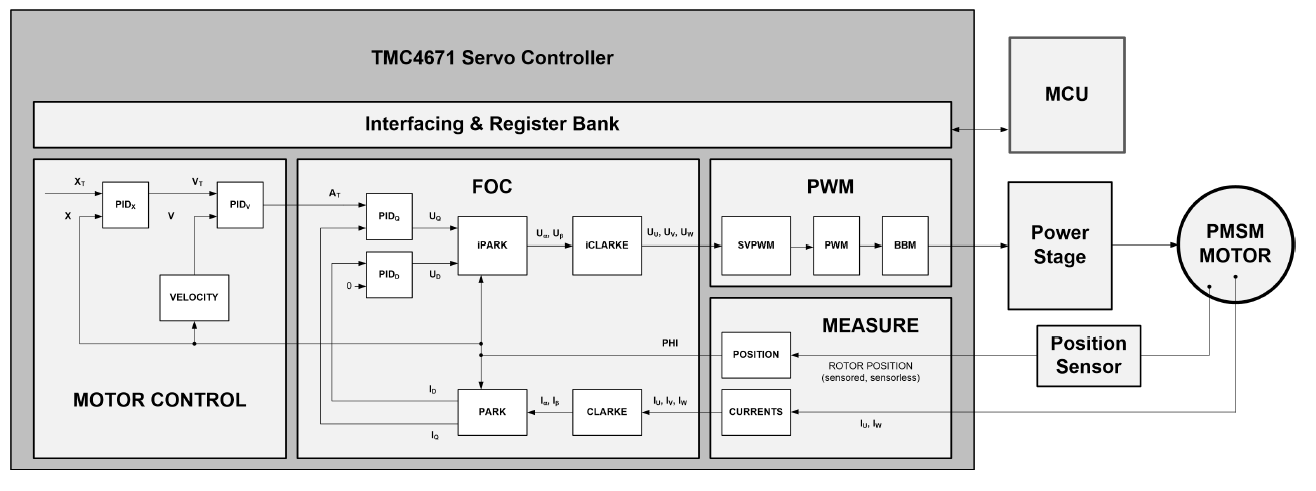
\includegraphics[width=\textwidth]{graphics/Blockdiagramm_TMC4671_FOC.png}
	\caption{Hardware FOC Blockdiagramm.\cite{trinamic_datasheet_2018}}
	\label{fig:Blockdiagramm_TMC4671_PID}
\end{figure}

 Ein DC-Motor wird vom Prinzip her wie in Abbildung \ref{fig:Blockdiagramm_TMC4671_PID_0} geregelt. Diese Abbildung zeigt einen vereinfachten Aufbau einer Antriebsregelung. Mittels den eingestellten PI-Parametern und dem eingestellten Betriebsmodus (Torque/Flux, Velocity, Position) werden beim TMC4671 die Abhängigkeiten der Regler geändert. Dies ist in Abbildung \ref{fig:Blockdiagramm_TMC4671_PID_1} ersichtlich. Im Drehmoment-Modus wird ``TARGET\_TORQUE`` als Ziel-Drehmoment verwendet. Im Geschwindigkeitsmodus wird das Zieldrehmoment vom Geschwindigkeits-PID-Regler vorgegeben. Im Drehmomentregler kann das maximale Drehmoment vorgegeben werden, welches auf den Motor gegeben wird. Eine detaillierte Übersicht der einzelnen Regler und deren Abhängigkeiten ist in Abbildung \ref{fig:Blockdiagramm_TMC4671_PID_2} zu finden.
\\

\begin{figure}[h!]
	\centering
	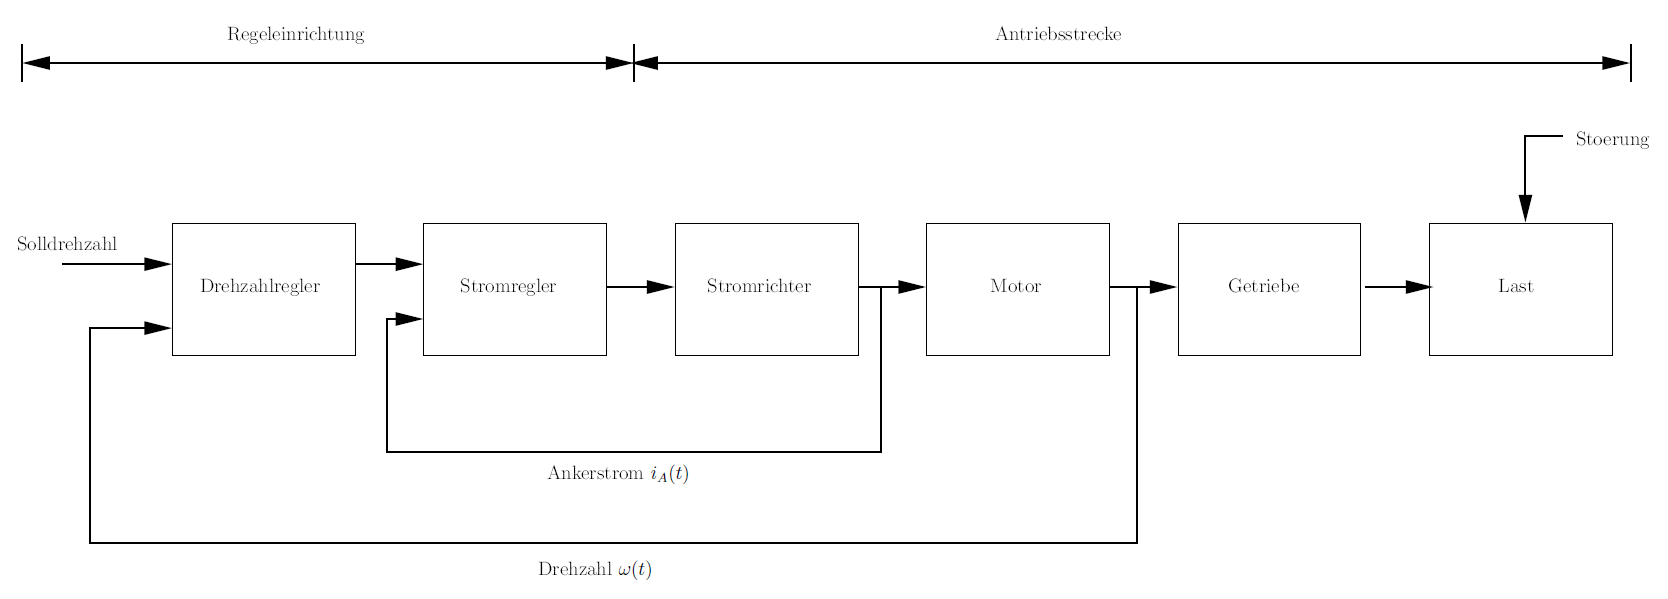
\includegraphics[width=\textwidth]{graphics/Prinzipieller_Antrieb_DC_Motor.png}
	\caption{Der Prinzipielle Aufbau einer Antriebsregelung für einen DC-Motor. 
	\cite{prof_dr-ing_raisch_stromregelung_nodate}
	}
	\label{fig:Blockdiagramm_TMC4671_PID_0}
\end{figure}

\begin{figure}[h!]
	\centering
	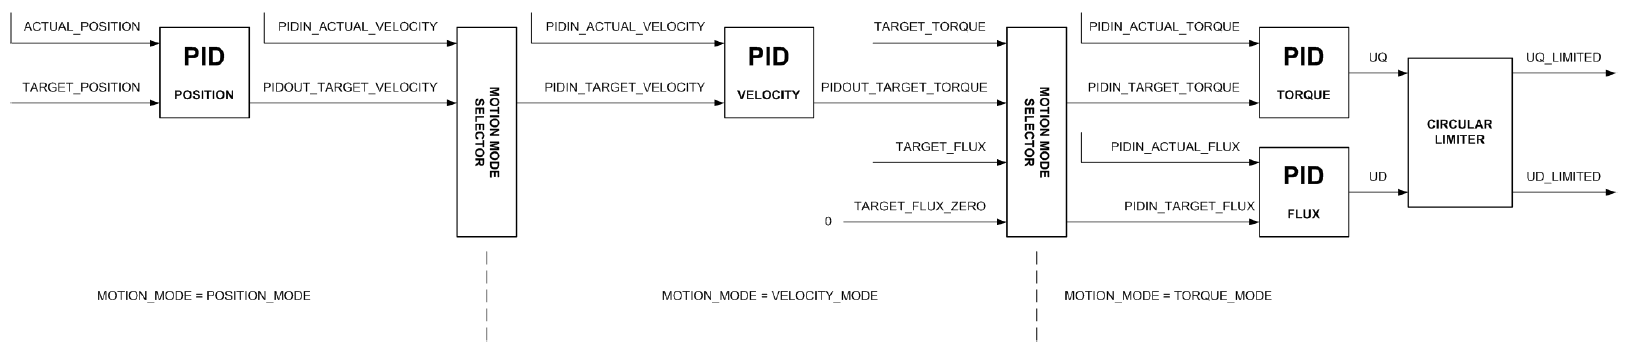
\includegraphics[width=\textwidth]{graphics/PI_Regler_Struktur_Gesamt.png}
	\caption{Abhängigkeiten der Regler.\cite{trinamic_datasheet_2018}}
	\label{fig:Blockdiagramm_TMC4671_PID_1}
\end{figure}

\newpage

\begin{figure}[h!]
	\centering
	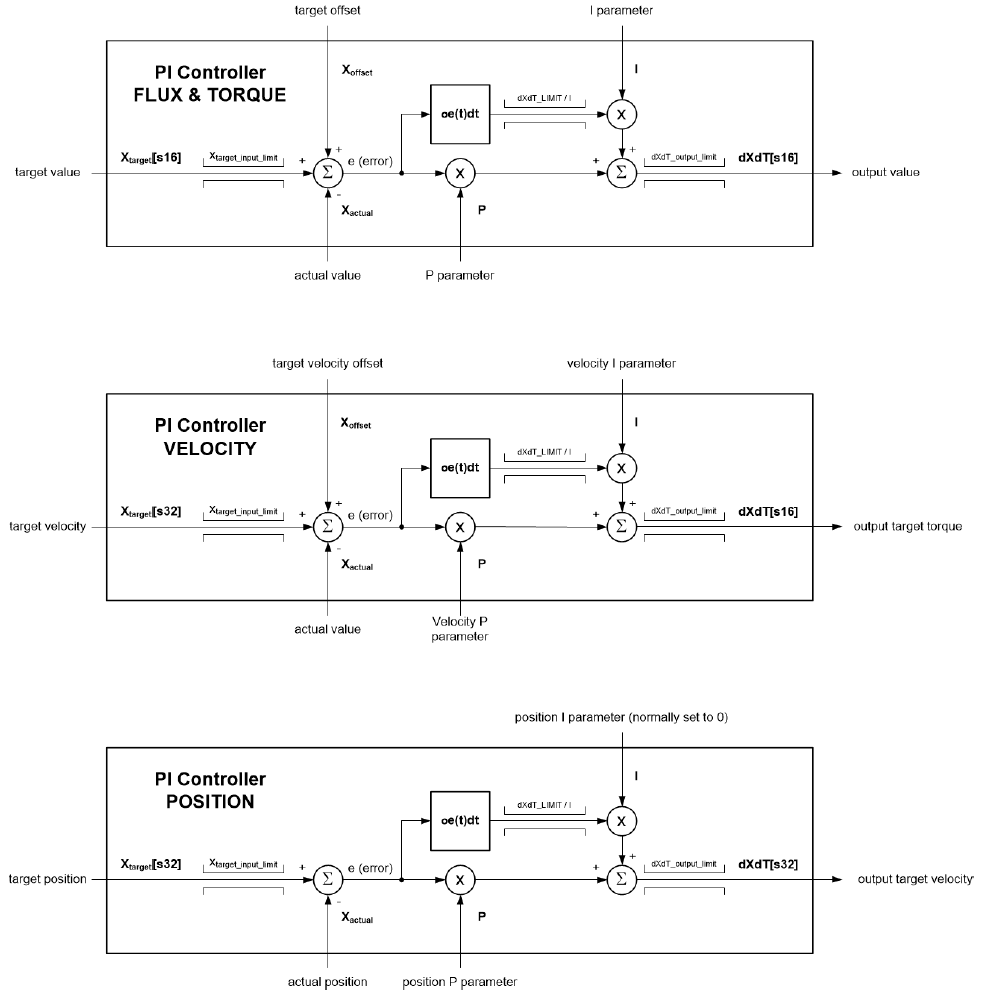
\includegraphics[width=\textwidth]{graphics/PI_Regler_Struktur.png}
	\caption{Die Reglerstufen im Detail. \cite{trinamic_datasheet_2018}}
	\label{fig:Blockdiagramm_TMC4671_PID_2}
\end{figure}

\newpage

Abbildung \ref{fig:PID_Target} zeigt, wie die Regelung im Positionsmodus eine Ziel-Position vorgibt (rot) und wie die aktuelle, gemessene Position tatsächlich ist (blau). Zu erkennen ist, dass die blaue Linie die Zielposition ziemlich steil anfährt und nicht überschiesst.

\begin{figure}[h!]
	\centering
	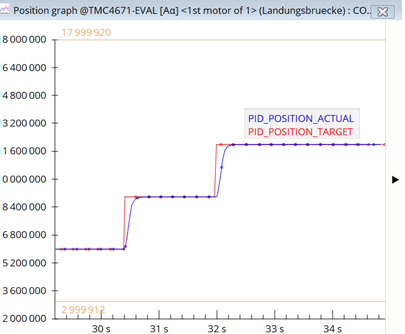
\includegraphics[width=0.6\textwidth]{graphics/PID_Target.png}
	\caption{Geschwindigkeitsregler mit Zielgraph und aktueller Graph. \cite{usb_von_herr_schleuniger_foc-motorenansteuerung_2019}}
	\label{fig:PID_Target}
\end{figure}
%\paragraph{Funktionsprinzip}\mbox{}\\

%In Abbildung \ref{fig:Blockdiagramm_TMC4671} ist ein vereinfachtes Block-Diagramm zu sehen, worin zu erkennen ist, wie die einzelnen Systemkomponenten zusammenhängen.


.
%\begin{tabbing}

%\parbox[t]{.1\textwidth}{

%MCU

%} \=\parbox[t]{.9\textwidth}{

%Kommuniziert über SPI mit dem Treiber. Die MCU schreibt und liest die Register des TMC4671. Dieser Teil wird auf dem EVAL-Board von der Landebrücke dargestellt. Bei der Cocktailmaschine wird dies der Atmega2560 sein.
%\\
%}\\

%\parbox[t]{.15\textwidth}{

%SPI

%} \> \parbox[t]{.9\textwidth}{

%Kommunikations-Interface des TMC4671. Der Treiber fungiert als Slave und decodiert die über die SPI-Schnittstelle übertragenen Daten.
%\\
%}\\

%\parbox[t]{.1\textwidth}{

%Registers

%} \>\parbox[t]{.9\textwidth}{

%Hier sind die Registerdaten gespeichert. Sie dienen dem Treiber als Parameter für dessen Funktion. Trinamic hat folgende Gruppierung festgelegt:

%\begin{multicols}{3}
%\begin{itemize}
%\item Informationen
%\item Allgemein
%\item ADC's
%\item Inputs/Outputs
%\item PWM
%\item Decoder ABN
%\item Hall digital
%\item Decoder analog
%\item PID-Regler
%\end{itemize}
%\end{multicols}

%}\\
%\parbox[t]{.15\textwidth}{
%FOC23
%} \>\parbox[t]{.9\textwidth}{
%Die FOC23-Engine führt den inneren Stromregelkreis für den Drehmomentstrom $I_Q$ und den Fluss-Strom $I_D$, einschließlich der erforderlichen Transformationen, welche noch erklärt werden. Programmierbare Begrenzer sorgen für einen sicheren Betrieb.
%\\
%}\\
%\parbox[t]{.15\textwidth}{
%Servo
%} \>\parbox[t]{.9\textwidth}{
%Mit 
%}\\
%\parbox[t]{.15\textwidth}{
%PWM
%} \>\parbox[t]{.9\textwidth}{
%Stellt Impulse für H-Brücke zur Verfügung.
%\\
%}\\
%\parbox[t]{.15\textwidth}{
%ADC
%} \>\parbox[t]{.9\textwidth}{
%Erlaubt analoge signale zu interpretieren
%}\\
%\parbox[t]{.15\textwidth}{
%Encoder
%} \>\parbox[t]{.9\textwidth}{
%Erlaubt, die Position des Rotors zu bestimmen
%}\\
%\parbox[t]{.15\textwidth}{
%Gate
%} \>\parbox[t]{.9\textwidth}{
%Steuert die Gates der Power-Stufe
%}\\
%\parbox[t]{.15\textwidth}{
%Power
%} \>\parbox[t]{.9\textwidth}{
%H-Brücke, wo der Motor angeschlossen wird.
%}\\
%\parbox[t]{.25\textwidth}{
%Current
%} \>\parbox[t]{.9\textwidth}{
%Feedback für Strom durch die Spule.
%}\\
%\parbox[t]{.25\textwidth}{
%BLDC
%} \>\parbox[t]{.9\textwidth}{
%Motor
%}\\
%\parbox[t]{.25\textwidth}{
%Encoder
%} \>\parbox[t]{.9\textwidth}{
%Resolver/ABN-Encoder
%}
%\end{tabbing}